\documentclass[11pt,a4paper]{article}

\usepackage{../../templates/style}

\begin{document}

\begin{problem}{Sushi}{standard input}{standard output}{4 second}{16 megabytes}

\textit{Benz Blaho} ได้ทำการสั่งซูชิชั้นสูงเข้ามารับประทานในร้านอาหารร้านหนึ่งใกล้โรงเรียน

ซูชิชั้นสูงมีลักษณะเป็นแท่งห่อสาหร่ายขนาดยาว $n$ หน่วย ซึ่งยังไม่ได้ตัด (ดูภาพประกอบ) แต่ทางร้านได้ทำรอยสำหรับตัดมาให้ทั้งสิ้น $m$ รอย คือรอย $R_1,R_2,…,R_m$


\begin{figure}[!h]
\centering
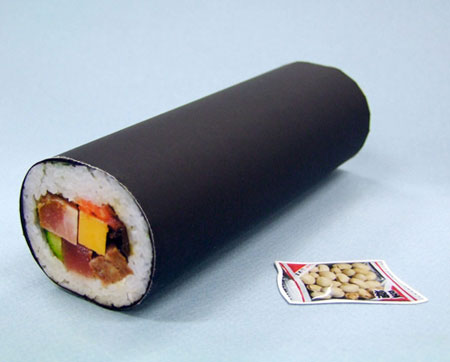
\includegraphics[width=0.4\textwidth]{../latex/img/1148/1148-1.jpg}
\captionsetup{justification=centering}
\caption*{ที่มา: \url{http://lh3.ggpht.com/\_4MUf6T4VzPw/TSyffZBh72I/AAAAAAAASqo/u9OMw2jTRU8/ehou-maki-papercraft-sushi-roll.jpg}}

\end{figure}

\textit{Benz Blaho} มีเพื่อนทั้งสิ้น $k$ คน และต้องการจะแบ่งซูชิที่เขาสั่งมานั้นให้กับเพื่อนๆของเขาทุกคน (ทุกคนจะต้องได้กินซูชิ) เพื่อนแต่ละคนนั้นจะมีค่าความชอบซูชิที่แตกต่างกัน โดยเพื่อนคนที่ $i$ จะมีค่าความชอบซูชิ $P_i$ หากเพื่อนคนที่มีค่าความชอบซูชิ $x$ ได้กินซูชิความยาว $y$ \textit{Benz Blaho} จะได้รับความสุข $x \times y$ หน่วย

          อย่างไรก็ตาม เพื่อนของ \textit{Benz Blaho} ค่อนข้างจะเรื่องมากเอาการ พวกเขาต้องการให้ \textit{Benz Blaho} วางแผนการตัดซูชิก่อนทำการตัดจริง โดยการเลือกรอยตัดมา $k-1$ รอยที่จะใช้ตัด และเมื่อทำการตัดแล้ว เพื่อนคนที่ $1$ จะได้กินซูชิชิ้นซ้ายสุด เพื่อนคนที่ $2$ จะได้กินซูชิชิ้นถัดไป …. เพื่อนคนที่ $k$ จะได้กินซูชิชิ้นขวาสุด
          
\bigskip
\underline{\textbf{โจทย์}}  จงเขียนโปรแกรมเพื่อหาวิธีการแบ่งซูชิสำหรับ \textit{Benz Blaho} เพื่อให้เขาได้รับค่าความสุขรวมมากที่สุด


\InputFile

\textbf{บรรทัดแรก} รับจำนวนนับ $n, m, k$  $( 1 \leq n \leq 1\,000\,000; 1 \leq k \leq m \leq 20\,000 )$

\textbf{บรรทัดที่สอง} รับจำนวนนับ $m$ จำนวน คือ $R_1$ $R_2$ $…$ $R_m$ $( 1 <  R_1 < R_2 < … < R_m < n )$ แทนระยะของรอยตัดแต่ละรอย วัดจากขอบซ้ายสุดของซูชิ

\textbf{บรรทัดที่สาม} จำนวนนับ $k$ จำนวน คือ $P_1$ $P_2$ $…$ $P_m$ $( 1 \leq P_i \leq 1\,000 )$ แทนค่าความชอบซูชิของเพื่อนแต่ละคน


\OutputFile

\textbf{มีบรรทัดเดียว} ระบุค่าความสุขรวมมากที่สุดที่ \textit{Benz Blaho} จะได้รับจากการแบ่งซูชิให้เพื่อนทั้ง $k$ คน

\Examples

\begin{example}
\exmp{10 5 3
1 3 5 8 9 
4 2 2}{36}%
\exmp{10 5 3
2 4 6 8 9 
4 3 9}{68}%
\end{example}


\Source

สรวิทย์  สุริยกาญจน์ ( PS.int )

ศูนย์ สอวน. โรงเรียนมหิดลวิทยานุสรณ์

นักแสดง :  \url{https://www.facebook.com/benz.beeb}


\end{problem}

\end{document}